\subsection{Data outline}
In order to get a preliminary idea of the raw data, the 5 different values of the relative spectral intensity were plotted against the wavelength in nm,   as can be seen in \textbf{Figure \ref{fig:Figure 1}}.
\begin{figure}[H]
    \centering
    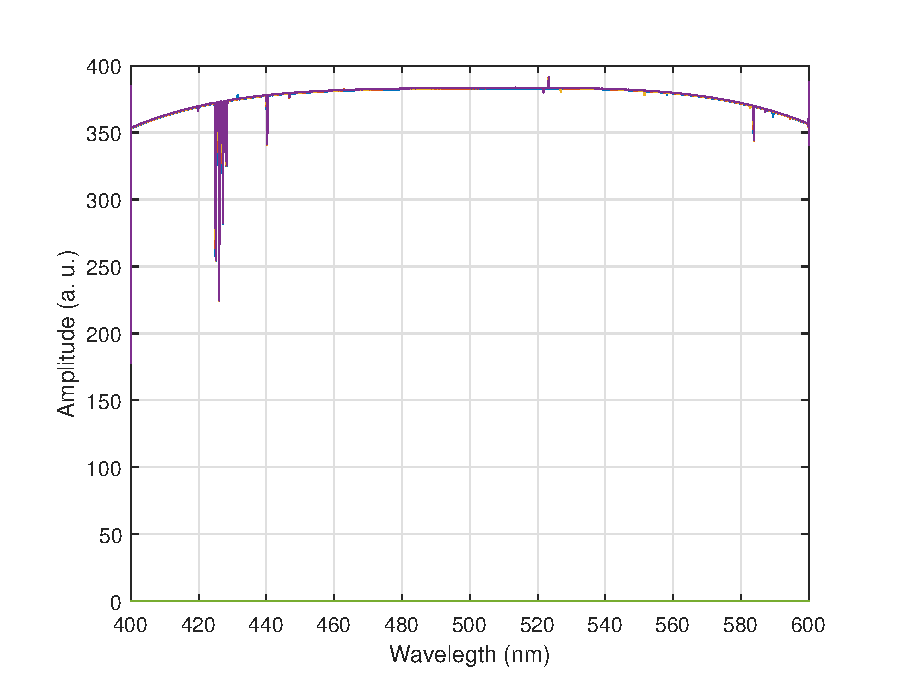
\includegraphics[width = 0.8\textwidth ]{figures/InitialPlot.eps}
    \caption{Initial plot. }
    \label{fig:Figure 1}
\end{figure}
Only 4 out of the 5 data-sets form the curve shown in the plot, as the 5th data-set is an array of broken data representing signal noise around the 0 intensity position. A zoomed out version of the data-set 5 can be seen in \textbf{Figure \ref{fig:Figure 2}}. This "broken" data was later used for noise estimations in the main spectrum. For the other four signals there is a presence of characteristic spectral peaks, both positive and negative, representing emission and absorption lines respectively. With the exception of a few spurious peaks, the majority appear consistently in each of the 5 data-sets, an example of some of these spurious peaks can be observed in \textbf{Figure\ref{fig:Figure 3}}. These also exhibit a measurable amount of random noise, as shown in \textbf{Figure \ref{fig:Figure 3}}, that is akin to the one observed in the 5th data-set. This noise can be due to spectrograph error, caused by variations in the light that goes through the prism and experimental noise\cite{Prisms}. Furthermore, there is a presence of strong intensity fluctuations around the first 10 and last 10 data-points in the spectrum. These are likely errors caused by the initiation and finalisation of the measurements, as seen in \textbf{Figure \ref{fig:Figure 4}}. After having determined this, a preliminary data cleanup is performed.


\begin{figure}[H]
    \centering
    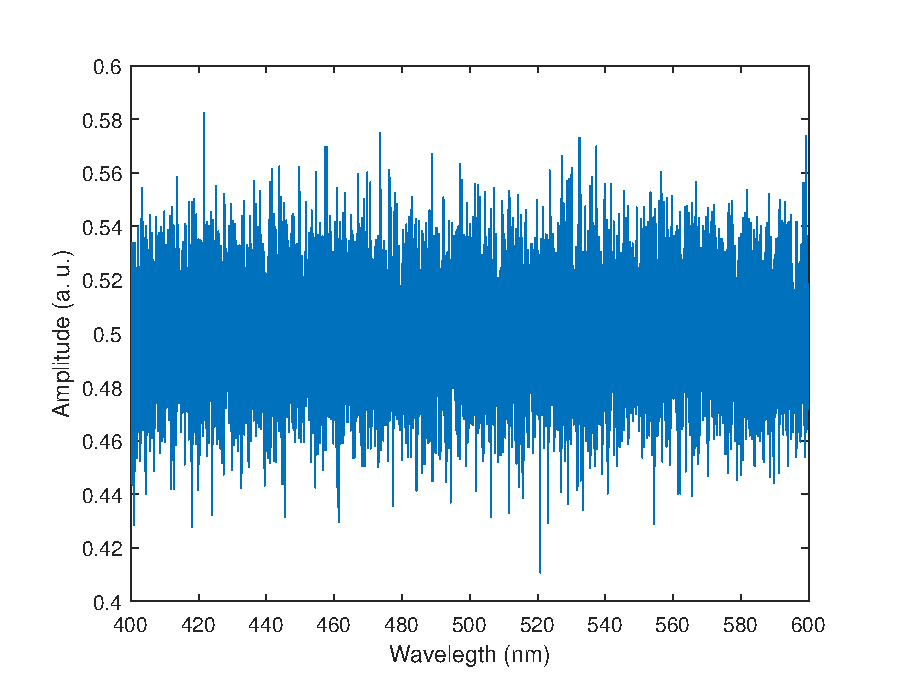
\includegraphics[width = 0.8\textwidth ]{figures/brokenData.eps}
    \caption{Broken data plot}
    \label{fig:Figure 2}
\end{figure}
\begin{figure}[H]
    \centering
    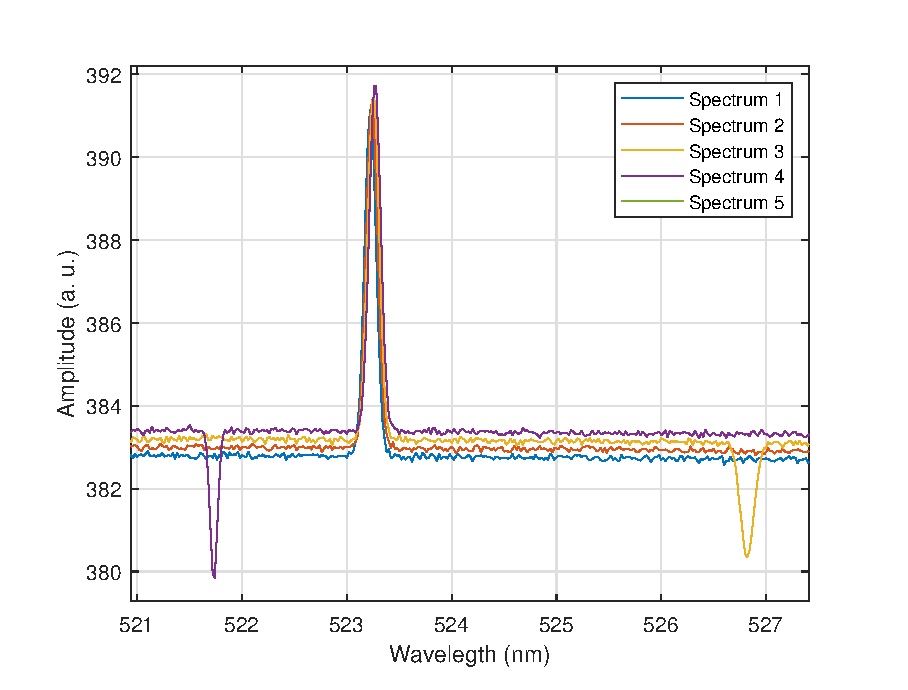
\includegraphics[width = 0.8\textwidth ]{figures/spurius_noise.eps}
    \caption{Spurious peaks and noise levels}
    \label{fig:Figure 3}
\end{figure}
\begin{figure}[H]
    \centering
    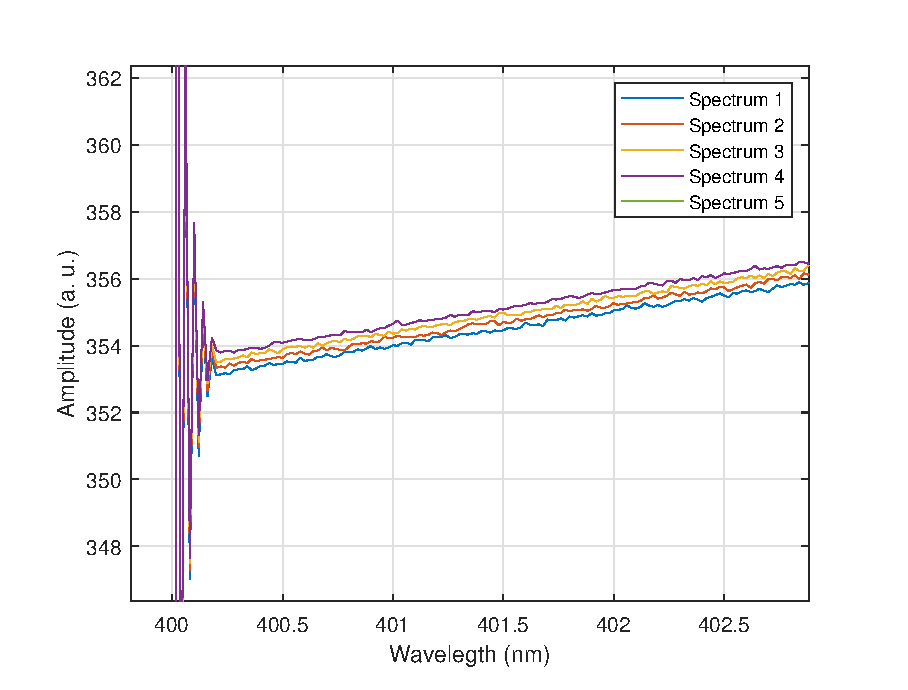
\includegraphics[width = 0.8\textwidth ]{figures/startError.eps}
    \caption{Start of measurement fluctuations}
    \label{fig:Figure 4}
\end{figure}
\subsection{Preliminary data processing}
First, the initialisation and finalisation fluctuation errors in the data are eliminated. For that, 12 points at the beginning of the data and at the end were removed, as a precaution measure to avoid interference with further data processing.


\subsection{Signal Characteristics}
The signal can be classified in different ways according to specific characteristics:
\begin{itemize}
    \item The signal is \textbf{deterministic}\cite{detSig}: The intensity of each wavelength in the emission spectrum depends on the specific conditions of the measurement and can be calculated precisely. This is despite random factors that cause uncertainty in the signal.
    \item The signal is \textbf{aperiodic}: The spectrum does not repeat itself or have a fixed time period
    \item The signal is \textbf{continuous}: The spectrum covers all wavelengths and is measured continuously without gaps or breaks
    \item The signal is \textbf{stationary}: The spectrum's properties are constant, showing equidistant samples at 0.02 nm.
    \item It is a \textbf{power signal}: The spectrum's intensity reflects the source's power output at each wavelength
    \item It is a \textbf{discrete-time signal}\cite{sigClas}:The values are at equally-spaced intervals along the x-axis.
\end{itemize}
\begin{table}[H]
    \centering
    \caption{Statistical properties of the signals (rounded up to 2nd decimal)}
    \begin{tabular}{|c|c|c|c|c|}
    \centering
    \textbf{} & \textbf{Mean} & \textbf{Var} &  \textbf{Skewness} & \textbf{Kurtosis}\\ \hline \hline
Spectrum 1   & 376.00    & 107.09    & -4.85 & 49.85 \\ \hline   
Spectrum 2   & 376.20    & 107.14    & -4.86 & 50.09 \\ \hline
Spectrum 3   & 376.39    & 107.06    & -4.86 & 50.09 \\ \hline
Spectrum 4   & 376.60    & 107.19    & -4.86 & 50.13 \\ \hline
Spectrum 5   & 0.5    & 4e-4    & 0.02 & 3.11
    \end{tabular}
    \label{tab:table1}
\end{table}
In \textbf{Table \ref{tab:table1}} can be observed basic statistical properties of the signal. As it can be observed, there is a continuous decrease of the Mean values in the signals for each data-set (excluding number 5). This could indicate a decrease in the luminous intensity perceived by the spectrograph in each subsequent measurement, perhaps even indicating that it has fallen out of range in measurement number 5. The variance, skewness and kurtosis do not show these differences and remain consistent across measurements. The variance indicates a dispersion in intensity across the whole spectrum, which includes the peaks of the spectral lines. This is the main source of the variance observed, as the residual noise is fairly small, as can be observed in the measurement number 5. The skewness is negative, indicating a general displacement of the higher intensities towards the lower wavelengths. This is also consistent with the higher peaks of the spectral lines that can be observed between 420 and 440 nm. The kurtosis values indicate substantial levels of peakness in the data, which are much more elevated than those of normal distributions, therefore proving that these sets of data-points are not normally distributed.

\subsection{Peak finding}
The spectral information from the data-sets 1 to 4 show a curvature, as observed in\textbf{ Figure \ref{fig:Figure 1}}. In order to accurately calculate the position of the spectral lines from these signals, this curvature has to be removed. In order to do that, a polynomial fit function that accurately describes the curvature has to be found, but Matlab 'polyfit' function showed inaccurate results due to the distorting effect of the spectral lines and other peaks in the data. Therefore, an algorithm for peak detection was used to identify and remove possible peaks from the continuum curve before fitting the polynomial. This algorithm returns the position and intensity of the peaks in all the spectra according to several parameters:

\begin{lstlisting}
numSpectra = 4; 
maxPeaksPerSpectrum = 10; % Pre-allocate space for performance
peaks = zeros(numSpectra, maxPeaksPerSpectrum);
peaksLoc = zeros(numSpectra, maxPeaksPerSpectrum);
negPeaks = zeros(numSpectra, maxPeaksPerSpectrum);
negPeaksLoc = zeros(numSpectra, maxPeaksPerSpectrum);

% Smooth the curve slightly for better 
% peak finding -currently 3-points moving average-
spectrum_smooth = smoothdata(spectrogram, 2, 'movmean', 3);

for i = 1:numSpectra
    % Find positive peaks in the spectrum
    [peaksFound, loc_posPeaks] = findpeaks(spectrum_smooth(i,:), 'MinPeakProminence', 0.5,'MinPeakHeight', 377.95,'Threshold', 0.02);
    numPeaksFound = numel(peaksFound);
    peaks(i, 1:numPeaksFound) = peaksFound;
    peaksLoc(i, 1:numPeaksFound) = loc_posPeaks;
        
    % Find negative peaks in the spectrum
    [negPeaksFound, loc_negPeaks] = findpeaks(-spectrum_smooth(i,:), 'MinPeakProminence', 0.2, 'Threshold', 0.005);
    numNegPeaksFound = numel(negPeaksFound);
    negPeaks(i, 1:numNegPeaksFound) = -negPeaksFound;
    negPeaksLoc(i, 1:numNegPeaksFound) = loc_negPeaks;
end
\end{lstlisting}
The results of the plotting can be observed in the \textbf{Figure \ref{fig:Figure 5}}.

\begin{figure}[H]
    \centering
    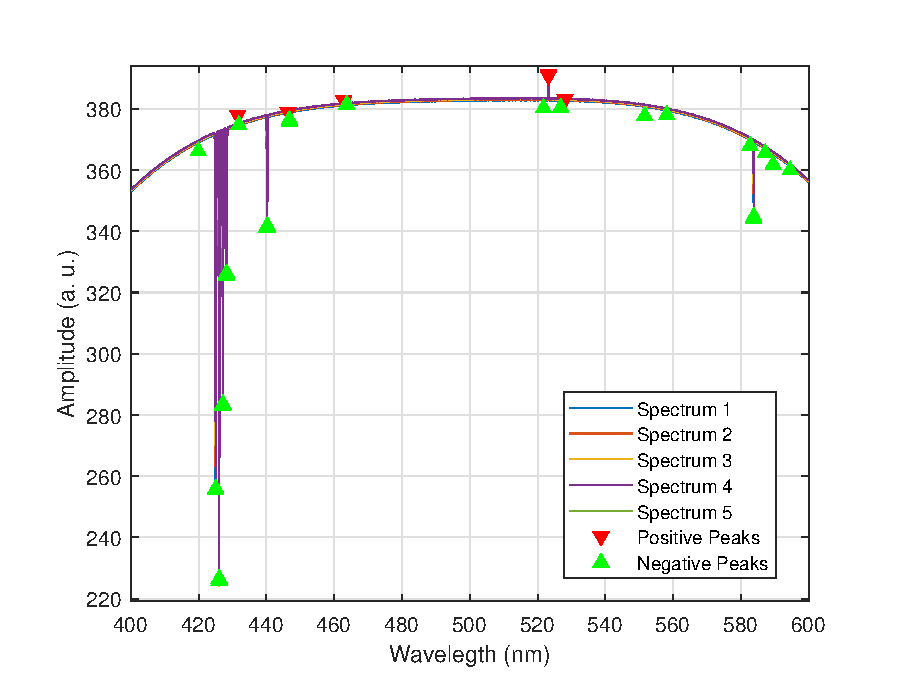
\includegraphics[width = 1\textwidth ]{figures/peakDetection1.eps}
    \caption{Location of detected peaks }
    \label{fig:Figure 5}
\end{figure}

\subsection{Calibration curve}
Based on the position of the peaks calculated in previous chapter, The continuum curve is split up into segments by removing a region of around 25 points before and after the peak maximum. The resulting data without the peaks is the calibration curve used to find the polynomial fit function for the spectra.
This curve is only used for finding the polynomial fit, and will not be used again elsewhere in the analysis.
The following Matlab algorithm was used:
\begin{lstlisting}
region_size = round(0.5 / wavelength_resolution);

for i = 1:numSpectra
    % Get the positive and negative peak locations for the current spectrum
    peak_locs = peaksLoc(i,:);
    peak_locs = peak_locs(peak_locs~=0); % Remove zero entries
    neg_peak_locs = negPeaksLoc(i,:);
    neg_peak_locs = neg_peak_locs(neg_peak_locs~=0); % Remove zero entries

    % Set values around the positive peaks to NaN in calibration_curve
    for j = 1:length(peak_locs)
        peak_loc = peak_locs(j);
        lower_bound = max(1, peak_loc - region_size);
        upper_bound = min(size(calibration_curve, 2), peak_loc + region_size);
        calibration_curve(i, lower_bound:upper_bound) = NaN;
    end
    
    % Set values around the negative peaks to NaN in calibration_curve
    for j = 1:length(neg_peak_locs)
        neg_peak_loc = neg_peak_locs(j);
        lower_bound = max(1, neg_peak_loc - region_size);
        upper_bound = min(size(calibration_curve, 2), neg_peak_loc + region_size);
        calibration_curve(i, lower_bound:upper_bound) = NaN;
    end
end
\end{lstlisting}
The visualisation of the calibration curve is in the following figure:(\textbf{Figure \ref{fig:Figure 6}})
\begin{figure}[H]
    \centering
    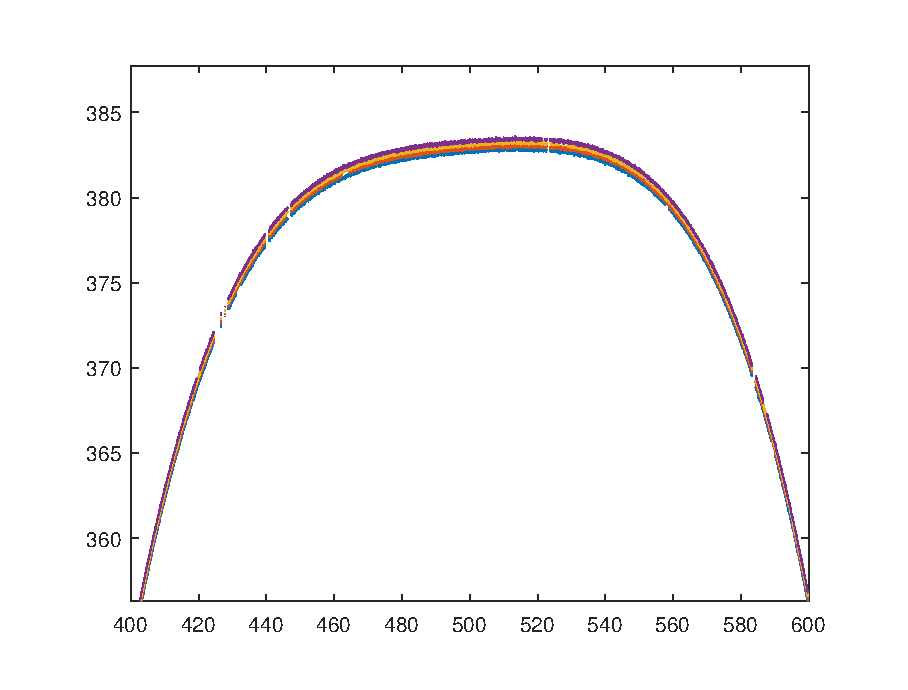
\includegraphics[width = 1\textwidth ]{figures/calibrationCurve.eps}
    \caption{Calibration Curve }
    \label{fig:Figure 6}
\end{figure}

Then, the empty gaps on the continuum are filled up by interpolating the empty values using interp1 linear interpolation as follows:
\begin{lstlisting}
current_row(nan_indices) = interp1(non_nan_indices, current_row(non_nan_indices), nan_indices, 'linear');
\end{lstlisting}
The result is a fully continuous curve (\textbf{Figure \ref{fig:Figure 7}}).
\begin{figure}[H]
    \centering
    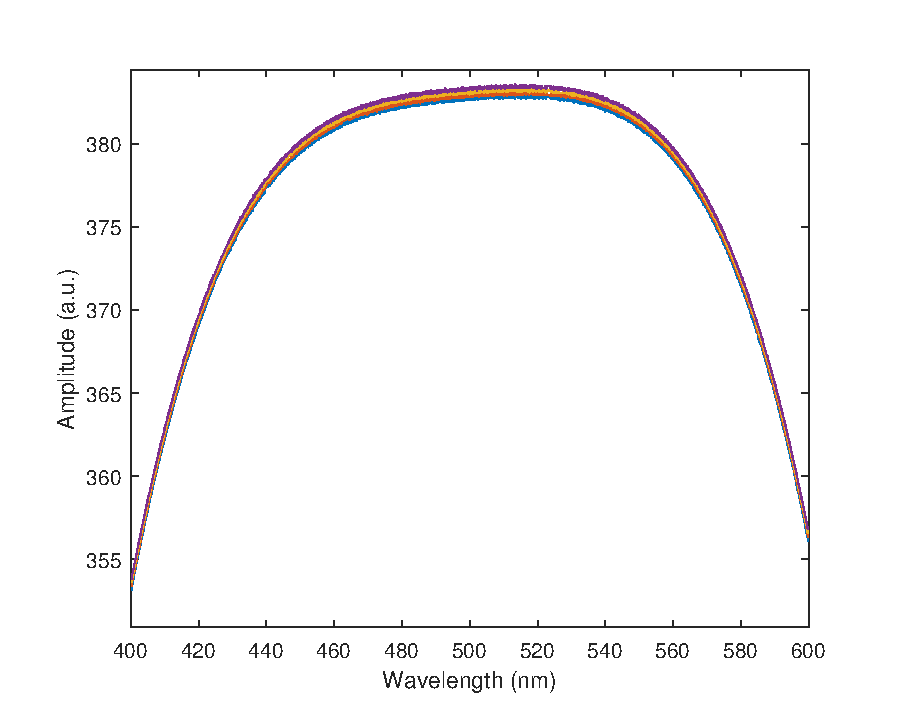
\includegraphics[width = 1\textwidth ]{figures/interpol_calibrationCurve.eps}
    \caption{Calibration Curve Interpolated }
    \label{fig:Figure 7}
\end{figure}

\subsection{Polynomial fit}
A polynomial fit of 4th degree is performed on the interpolated calibration curve. This allow us to obtain the parameters of the curve to correct the curvature of the signal. The following function 'polyfit'\cite{polyfit} was called in Matlab, and the results can be seen in \textbf{Figure \ref{fig:Figure 8}} as well as a zoomed-in version in \textbf{Figure \ref{fig:Figure 9}}.
\begin{lstlisting}
degree = 4;
p = polyfit(x(~isnan(y)), y(~isnan(y)), degree);
y_fit = polyval(p, x);
\end{lstlisting}
\begin{figure}[H]
    \centering
    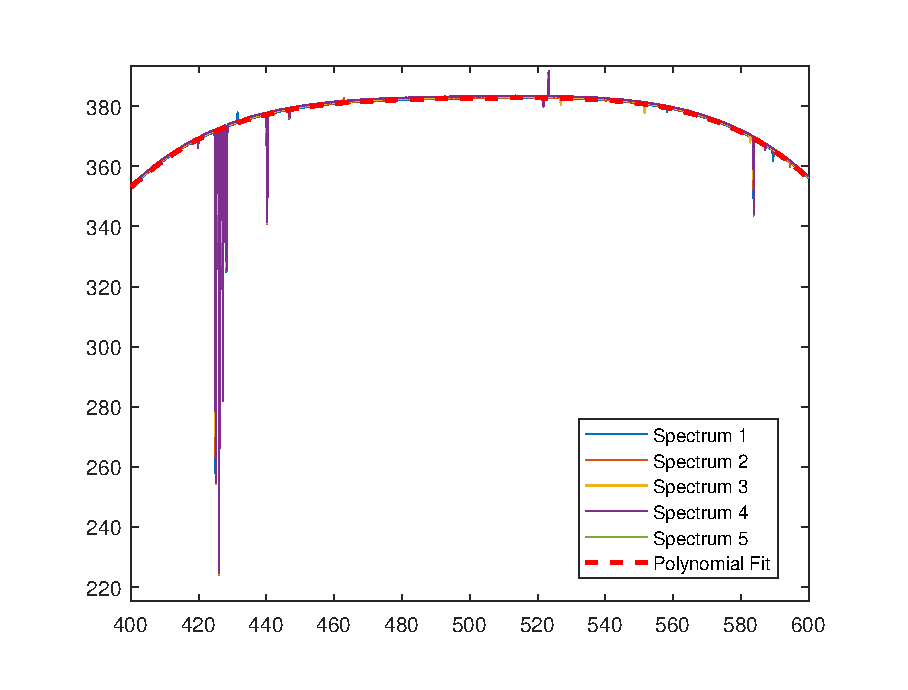
\includegraphics[width = 0.8\textwidth ]{figures/polyfit.eps}
    \caption{Polynomial fit of 4th degree on the calibration curve}
    \label{fig:Figure 8}
\end{figure}
\begin{figure}[H]
    \centering
    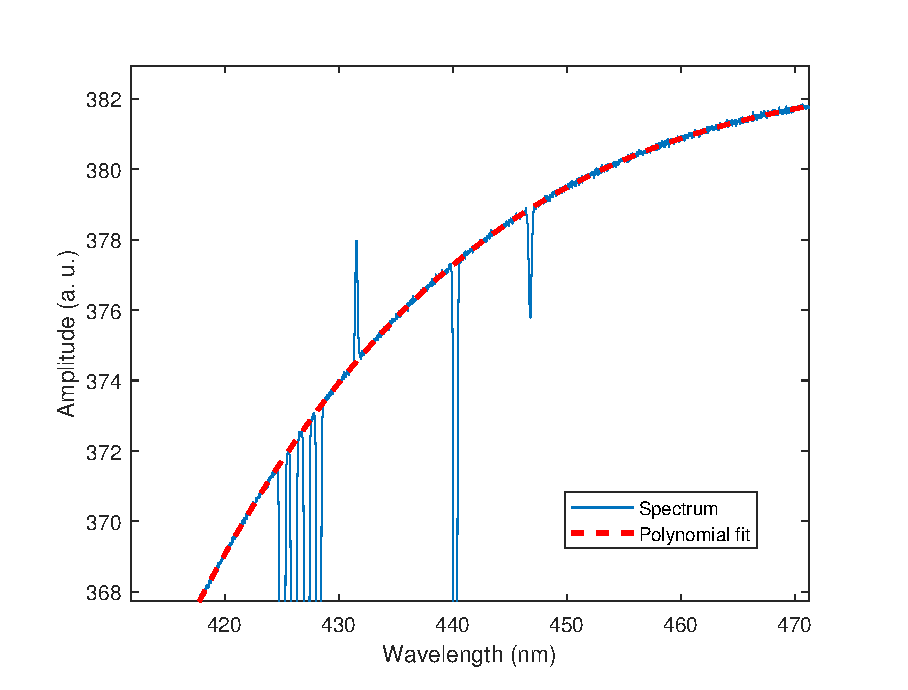
\includegraphics[width = 0.8\textwidth ]{figures/polyfit_zoom.eps}
    \caption{Polynomial fit zoom }
    \label{fig:Figure 9}
\end{figure}

\subsection{Curvature correction}
In order to correct the curvature of the continuum, I divided the entirety of the spectral data by the polynomial fit function. Then I detrended the signal by dividing it against its mean. This created a new corrected data for the 4 spectra, centered around 0, and can be observed in \textbf{Figure \ref{fig:Figure 10}}.

\begin{lstlisting}
corrected_signal = spectrogram ./ y_fit;
corrected_signal_detrended = bsxfun(@minus, corrected_signal, mean(corrected_signal, 2));
\end{lstlisting}

\begin{figure}[H]
    \centering
    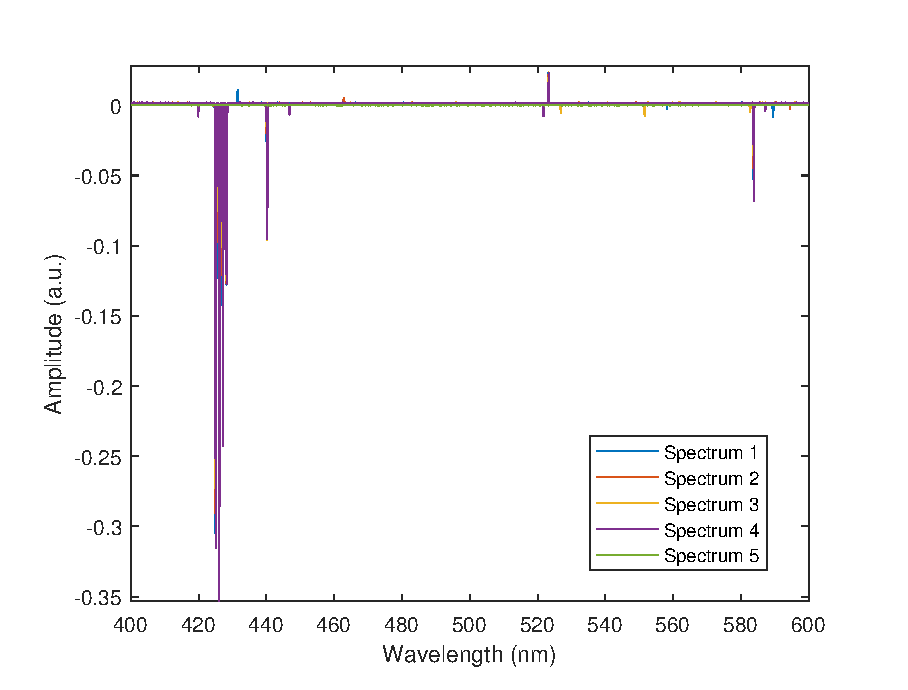
\includegraphics[width = 1\textwidth ]{figures/correctedSignal_detrended.eps}
    \caption{Corrected signal detrended}
    \label{fig:Figure 10}
\end{figure}

\subsection{Noise removal}
As mentioned in the Data outline, the data set number 5 contains seemingly broken data, but this could still be useful as it carries information about the background noise of the signals. This poses as an opportunity to further clean-up the spectral data of any random noise with the purpose to more accurately identify the spectral lines for element identification later on. Therefore I developed an algorithm to perform this cleaning.

\begin{itemize}
\item Subtracting the mean of data-set 5 from the rest of spectra
    \begin{lstlisting}
    cleaned_spectra = spectra - mean(spectra(5,:));
    \end{lstlisting}
    \item Calculate the noise threshold by obtaining absolute values of the data-set 5 and summing up the means
    \begin{lstlisting}
noise_threshold = max(abs(spectra(5,:)))+mean(cleaned_spectra(1:4,:),1)
\end{lstlisting}
    \item Set any values below the noise threshold to zero
    \begin{lstlisting}
for i=1:size(cleaned_spectra,1)-1
        for j=1:size(cleaned_spectra,2)
            if abs(cleaned_spectra(i,j)) < noise_threshold(i)
                cleaned_spectra(i,j) = 0;
            end
        end
    end
\end{lstlisting}
\end{itemize}

I also removed the spurious peaks such as the one shown in \textbf{Figure \ref{fig:Figure 3}}, by finding the peaks only present in one data-set, and setting them to zero.

\begin{lstlisting}
single_nonzero_cols = find(sum(cleaned_spectra(1:4,:)~=0,1)==1);
cleaned_spectra(1:4,single_nonzero_cols) = 0;
\end{lstlisting}

This results in a very clean signal in which the peaks of the spectral lines can be easily identified, as seeing in the detail against the previous noisy data in \textbf{Figure \ref{fig:Figure 11}}.

\begin{figure}[H]
    \centering
    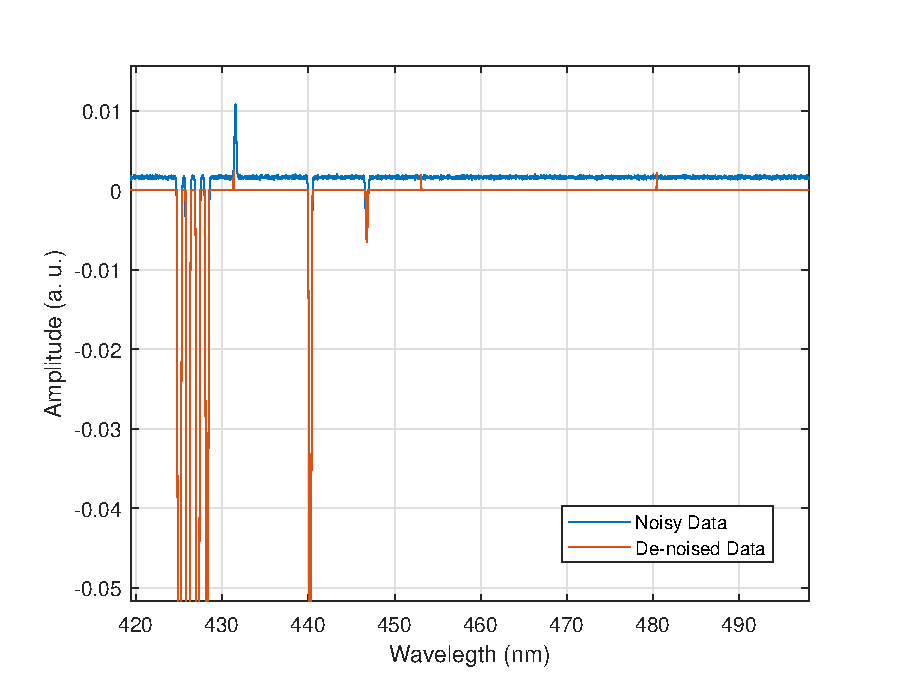
\includegraphics[width = 1\textwidth ]{figures/cleanedUpSpectra.eps}
    \caption{Cleaned-up data detail}
    \label{fig:Figure 11}
\end{figure}